\newcommand{\deadline}{07.07.2023}

\documentclass[11pt]{article}

\usepackage[exercise,ex]{custom_2.1}

\begin{document}

\section{Energie des Magentfeld}
\subsection{}
\begin{align*}
    L &= N\cdot U + l\\
    N &= \frac{L-l}{2\pi \cdot r}\\
    &\approx \frac{1500\u m - 1.8\u m}{2\pi \cdot 2.5\u{cm}}\\
    &\approx 9537.84
\end{align*}

\subsection{}
\begin{align*}
    B &= \mu_0 \frac {NI}l\\
    &\approx \munull \cdot \frac{9537.84 \cdot 350\u A}{1.8\u m}\\
    &\approx 2.34 \u T\\
    \\
    w &= \frac WV\\
    &= \frac 12 \frac{\mu_0 N^2 F }lI^2 \cdot \frac{1}{F l}\\
    &= \frac 1{2\mu_0} \hug{\mu_0 \frac {NI}l}^2 \\
    &= \frac{B^2}{2\mu_0}\\
    &\approx \frac{2.34^2 \u T^2}{2\cdot \munull}\\
    &\approx 2.17\megad \ufrac{J}{m^3}\\
    \\
    E &= \frac 12 L I^2\\
    L &= \frac{\mu_0 N^2 F }l\\
    &= \frac{\mu_0 F(L-l)^2}{4l\pi^2 r^2 }\\
    E &= \frac{\mu_0 F(L-l)^2}{8 l\pi^2 r^2 } I^2\\
\end{align*}

\subsection{}
\begin{align*}
    W_{total} &= w \cdot V\\
    &= w \cdot \frac12 \pi r^2 \cdot l \\
    &\approx 2.17\megad \ufrac{J}{m^3} \cdot \frac12 \pi \cdot 2.5^2\u{cm}^2 \cdot 1.8 \u m \\
    &\approx 3.84\u{kJ}
\end{align*}

\section{L-C-Tief- und -Hochpass}
\subsection{}
\begin{adjustwidth}{20pt}{}
    Impedanz des Kondensators:
\end{adjustwidth}
\begin{align*}
    U &= \frac{Q}{C}\\
    \dot {\un u} &= \frac{\un i}{C}\\
    j\omega\cdot {\un u} &= \frac{\un i}{C}\\
    \un Z &= \frac{\un u}{\un i} = \frac{1}{j \omega C}\\
\end{align*}
\begin{adjustwidth}{20pt}{}
    Impedanz der Spule:
\end{adjustwidth}
\begin{align*}
    U &= L \dot I\\
    \un u &= L \cdot j\omega \cdot \un i\\
    \un Z &= \frac{\un u}{\un i} = j\omega L \\
\end{align*}
\begin{adjustwidth}{20pt}{}
    Frequenzgang:
\end{adjustwidth}
\begin{align*}
    \frac{\un {u_a}}{\un {u_e}} &= \frac{\un {Z_a}}{\un {Z_e}}\\
    &= \frac{\frac{1}{j \omega C}}{\frac{1}{j \omega C} + j\omega L}\\
    &= \frac{\frac{1}{\omega C}}{\frac{1}{\omega C} - \omega L}\\
    &= \frac{1}{1 - \omega^2 L C}\\
    &= \frac{1}{1 - \frac{\omega^2}{\omega_0^2}}\\
\end{align*}

\subsection{}
\begin{align*}
    \frac{\un {u_a}}{\un {u_e}} &= \frac{\un {Z_a}}{\un {Z_e}}\\
    &= \frac{j \omega L}{\frac{1}{j \omega C} + j\omega L}\\
    &= \frac{1}{1 - \frac{1}{\omega^2 L bC}}\\
    &= \frac{1}{1 - \frac{\omega_0^2}{\omega^2}}\\
\end{align*}

\begin{adjustwidth}{20pt}{}
    Die Ausgangsspannung kann, ohne die Energieerhaltung zu verletzten, größer werden 
    als die Eingangsspannung, da in dem Kondensator und in der Spule Energie temporär 
    in den Feldern gespeichert wird und anschließend auch wieder in den Spromkreis 
    gespeist werden kann wodurch ein kurzer (prinzipiell beliebig großer) peak in der 
    Spannung/Storm entstehen kann. Die Ausgangs Spannung kann auch permanent höher sein als
    die Eingangsspannung, jedoch ist dann der fließende Strom geringer.
\end{adjustwidth}
\begin{figure}[h]
    \centering
    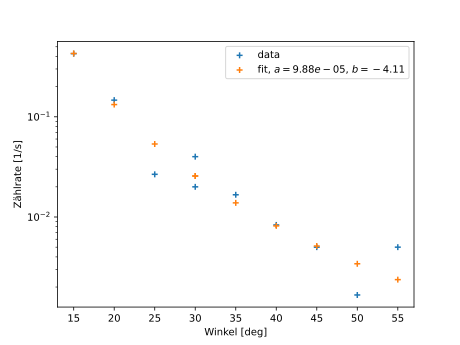
\includegraphics[width=0.7\textwidth]{2.png}
    \caption{$\substack{\te{X-Achse: }\frac{\omega}{\omega_0}\te{, Y-Achse: }\frac{U_a}{U_e}\\ \te{grün: erste Schaltskizze, blau: zweite Schaltskizze}}$}
\end{figure}

\section{Transformator}
\subsection{}
\begin{align*}
    \un {u_n} &= \sum_m L_m \deriv{\un{i_m}}{t}\\
    \un {u_n} &= N \cdot \dot \Phi\\
    &= N_n(\dot \Phi_{nn} + \dot \Phi_{mn})\\
    &= N_n\hug{A \dot B_{n} + A \dot B_{m}}\\
    &= N_n\hug{A \cdot \mu_0 \mu_r \frac{N_n}{l} \dot i_n + A \cdot \mu_0 \mu_r \frac{N_m}{l} \dot i_m}\\
    &= \underbrace{\mu_0 \mu_{r,n} \frac{N_n^2 A }{l}}_{L_n} \dot i_n + \underbrace{\mu_0 \mu_{r,mn} \frac{N_n N_m A}{l}}_{L_{nm}} \dot i_m\\
    &= L_n\dot i_n + L_{nm} \dot i_m\\
    &= j \omega L_n i_n + j \omega L_{nm}i_m\\
    &\rightarrow\begin{cases}
        u_1 = j \omega L_1 i_1 + j \omega L_{12} i_2\\
        u_2 = Z i_2 = j \omega L_2 i_2 + j \omega L_{12} i_1\\
    \end{cases}\\
    &\rightarrow\begin{cases}
        u_1 = j \omega L_1 i_1 + j \omega L_{12} i_2\\
        i_2 = \frac{j \omega L_{12} }{ Z - j \omega L_2}i_1\\
    \end{cases}\\
    &\rightarrow\begin{cases}
        u_1 = j \omega  \hug{L_1 +  \frac{j \omega L_{12}^2 }{ Z - j \omega L_2}}i_1\\
        \ \ \ \ = \frac{j \omega L_1 Z + \omega^2 (L_1 L_2 - L_{12}^2)}{Z - j \omega L_2} i_1\\
    \end{cases}\\
    &\rightarrow\begin{cases}
        u_1 = \frac{j \omega L_1 Z + \omega^2 (L_1 L_2 - L_{12}^2)}{Z - j \omega L_2} i_1\\
        u_1 = - \frac{j \omega L_1 Z + \omega^2 (L_1 L_2 - L_{12}^2)}{i\omega L_{12}} i_2
    \end{cases}\\
    \frac{i_2}{i_1} &=-  \frac{j\omega L_{12}}{Z + j \omega L_2}\\
    \frac{u_2}{i_1 Z} &=-  \frac{j\omega L_{12}}{Z + j \omega L_2}\\
    \frac{u_2}{u_1} &= -\frac{j\omega L_{12} Z}{j\omega L_1 Z + \omega^2 (L_{12}^2-L_1 L_2)}
\end{align*}

\subsection{}
\begin{align*}\frac{a + bi}{c+ di} &= \frac{(a + bi)(c+id)}{c^2+ d^2}\\
    &= \frac{(ac - bd) + i(ad + bc)}{c^2+ d^2}\\
    \abs{\frac{a + bi}{c+ di}}&= \frac{ac - bd}{c^2+ d^2}\\
    \abs{\frac{a + bi}{c+ di}} /\abs{\frac{e + fi}{c+ di}}&= \frac{ac - bd}{c^2+ d^2} \frac{c^2+ d^2}{ec - fd}\\
    &= \frac{ac - bd}{ec - fd}\\
    i_1 &= \frac{Z - j \omega L_2}{j \omega L_1 Z + \omega^2 (L_1 L_2 - L_{12}^2)} u_1\\
    i_2 &= \frac{-j\omega L_{12}}{j \omega L_1 Z + \omega^2 (L_1 L_2 - L_{12}^2)} u_1\\
    \frac{\abs{i_2}}{\abs{i_1}} &=  \frac{\omega^2 Z (L_1 L_2 - L_{12}^2) + \omega^2 Z L_1 L_2}
    {\omega ^2 Z L_1 L_{12}}\\
    &=  \frac{(L_1 L_2 - L_{12}^2) +  L_1 L_2}
    {L_1 L_{12}}\\
    &= \frac{{\mu_0 \mu_{r} \frac{N_1^2 A }{l} \cdot \mu_0 \mu_{r} \frac{N_2^2 A }{l}} 
    - \mu_0^2 \mu_{r}^2 \frac{N_1^2 N_2^2 A^2 }{l^2} +  
    \mu_0 \mu_{r} \frac{N_1^2 A }{l} \cdot \mu_0 \mu_{r} \frac{N_2^2 A }{l}}
    {\mu_0 \mu_{r} \frac{N_1^2 A }{l}\cdot  \mu_0 \mu_{r} \frac{N_1 N_2 A }{l}}\\
    &= \frac{N_1^2 \cdot N_2^2}
    {N_1^2\cdot N_1 N_2}\\
    &= \frac{N_2}{N_1}\\ 
\end{align*}

\subsection{}
\begin{align*}
    \frac{u_2}{u_1} &= -\frac{j\omega L_{12} Z}{j\omega L_1 Z + \omega^2 (L_{12}^2-L_1 L_2)}\\
    &= -\frac{j\omega L_{12} \frac{1}{j \omega C}}{j\omega L_1 \frac{1}{j \omega C} + \omega^2 (L_{12}^2-L_1 L_2)}\\
    &= -\frac{L_{12}/C}{L_1 /C + \omega^2 (L_{12}^2-L_1 L_2)}\\
    &\approx - 1.5
\end{align*}

\section{Schwingkreise}
\subsection{}
\begin{adjustwidth}{20pt}{}
    Aus dem Aufbau folgt mit der Knotenregel direkt:
\end{adjustwidth}
\begin{align*}
    &\rightarrow \begin{cases}
        0 = I_R + I_C + I_L\\
        U_R=U_C=U_L \hat = U\\
    \end{cases}
\end{align*}
\begin{align*}
    0 &= I_R + I_C + I_L\\
    0 &\eq \frac{U}{R} + \dot Q + \frac 1L \int U\dt \\
    0 &= \frac{Q}{R C} + \dot Q  + \frac 1{LC} \int Q\dt \\
    0 &= \ddot Q + \frac{\dot Q}{R C} + \frac Q{LC} \\
\end{align*}
\begin{adjustwidth}{20pt}{}
    \con denn \(\begin{cases}
        U_L = L \dot I_L\\
        I_L = \frac 1L \int U_L\dt\\
    \end{cases}\)
\end{adjustwidth}

\subsection{}
\begin{align*}
    \un Y_{ges} &= \un Y_{R} +\un Y_{C} +\un Y_{L}\\
    &= \frac{1}{R} + j \omega C +  \frac{1}{j\omega L }\\
    \un Z_{ges} &= \frac{1}{ \frac{1}{R} + j \hug{\omega C - \frac{1}{\omega L }}}\\
    &= \frac{\frac{1}{R} - j \hug{\omega C - \frac{1}{\omega L }}}{ \frac{1}{R^2} + \hug{\omega C - \frac{1}{\omega L }}^2}\\
    Z &= \abs{\un Z_{ges}} = \sqrt{\hug{\frac{\frac{1}{R}}{ \frac{1}{R^2} + \hug{\omega C - \frac{1}{\omega L }}^2}}^2
     + \hug{ \frac{\hug{\omega C - \frac{1}{\omega L }}}{ \frac{1}{R^2} + \hug{\omega C - \frac{1}{\omega L }}^2}}^2}
\end{align*}
\begin{align*}
    Y_C &= \\
    U &= \frac QC\\
    0 &= \ddot Q + \frac{\dot Q}{R C} + \frac Q{LC} \\
    0 &= \ddot I + \frac{\dot I}{R C} + \frac I{LC} \\
    0 &\eq -\omega^2\cdot \un i + j\omega\cdot\frac{\un i}{R C} + \frac {\un i}{LC} \\
    Z &= \frac{U}{I}
\end{align*}
\begin{adjustwidth}{20pt}{}
    \con da \(\un i = \i e^{j(\omega t + \phi)} \rightarrow \dot{\un i} = j\omega \cdot \i e^{i(\omega t + \phi)}\) 
\end{adjustwidth}

\subsection{}
\begin{adjustwidth}{20pt}{}
    Ansatz \(\rightarrow\) Exponentialfunktion :
\end{adjustwidth}
\begin{align*}
    Q &= c e^{\lambda t} \notethat c\in\C\\
    0 &= \ddot Q + \frac{\dot Q}{R C} + \frac Q{LC}\\
    0 &= \lambda^2 + \frac{\lambda}{R C} + \frac 1{LC}\\
    \lambda &= -\frac{1}{2 R C} \pm \sqrt{\frac{1}{4R^2 C^2} - \frac 1{LC}}\\
    Q(t) &= e^{-\frac t{2RC}} \hug{c_1 e^{t\sqrt{\frac{1}{4R^2 C^2} - \frac 1{LC}}}
    + c_2 e^{-t\sqrt{\frac{1}{4R^2 C^2} - \frac 1{LC}}}}\\
\end{align*}
\begin{align*}
    A &= \frac 1{2RC}\\
    B &= \sqrt{A^2 - \frac 1{LC}}\\
    Q(t) &= e^{-A t} \hug{c_1 e^{B t}+ c_2 e^{-B t}}
\end{align*}
\begin{align*}
    Q_{B\in\R}(t) &\equiv Q_\R(t)= e^{-A t} \hug{c_1 e^{B t}+ c_2 e^{-B t}}\\
    Q_\R(0) &= Q_0\\
    \dot Q_\R(0) &= 0\\ 
    Q_0 &= c_1 + c_2 \\
    0 &= B(c_1 - c_2) -A(c_1+c_2)\\
    0 &= B(2c_1 - Q_0) -A Q_0\\
    c_1 &= \frac {Q_0}2\hug{\frac AB + 1}\\
    c_2 &= Q_0 - \frac {Q_0}2\hug{\frac AB + 1}\\
    &= \frac {Q_0}2\hug{1 - \frac AB}
\end{align*}
\begin{figure}[h]
    \centering
    \includegraphics[width=0.7\textwidth]{0.024.png}
    \caption{\(R=0.024 \,\Omega\)}
\end{figure}

\begin{figure}[h]
    \centering
    \includegraphics[width=0.7\textwidth]{0.24.png}
    \caption{\(R=0.24 \,\Omega\)}
\end{figure}
\begin{align*}
    Q_{B\in\C}(t) &= e^{-A t} \hug{c_1 (\cos(\abs B t) + i\sin(\abs B t)) + c_2 (\cos(\abs B t) - i\sin(\abs B t))}\\
    \Re \hug{Q_{B\in\C}(t)} & \equiv Q_\C(t)= e^{-A t} \hug{c_{11}\cos(\abs B t) - c_{12}\sin(\abs B t) + c_{21} \cos(\abs B t) + c_{22}\sin(\abs B t)}\\
    &= e^{-A t} \hug{\hug{c_{11} + c_{21}}\cos(\abs B t) + (c_{22}- c_{12})\sin(\abs B t)}\\
    &= e^{-A t} \hug{c_1\cos(\abs B t) + c_2\sin(\abs B t)}\\
    Q_\C(0)&= Q_0\\
    \dot Q_\C(0)&= 0\\
    Q_0 &= c_1\\
    0 &= -A c_1 + \abs B c_2\\
    c_2 &= Q_0 \frac{A}{\abs B}
\end{align*}

\begin{figure}[h]
    \centering
    \includegraphics[width=0.7\textwidth]{2.4.png}
    \caption{\(R=2.4 \,\Omega\)}
\end{figure}

\end{document}   
